\section{Overzicht van bestaande datasets en annotatietechnieken}

\subsection{Beschikbaarheid van publieke datasets}

Zoals al eerder vermeld, is er voor het trainen van een objectdetectiemodel een substantiële hoeveelheid gelabelde data nodig. Tegenwoordig worden veel datasets -- zo goed als volledig geprepareerd voor het trainen van ML-modellen -- online aangeboden onder een vrije licentie. Dit zorgt ervoor dat de datasets opnieuw gepubliceerd en hergebruikt mogen worden met weinig tot geen beperkingen. Het concept van \emph{Open Data} wordt de laatste jaren steeds populairder, aangezien onderzoek zich hoe langer hoe meer ook naar het internet verplaatst. \autocite{Murray_Rust_2008} \\

Platformen zoals \href{https://www.kaggle.com/datasets}{Kaggle} of \href{https://huggingface.co/datasets}{Hugging Face} hebben zich gespecialiseerd in het verspreiden van deze open datasets en kunnen rekenen op een hele community van gebruikers om deze datasets te uploaden naar hun platformen. Ook verschillende overheidsorganisaties en onderzoeksinstellingen maken veel van hun data openbaar. Voorbeelden hiervan zijn \href{https://data.europa.eu/}{data.europa.eu} voor het dataplatform van de Europese Unie, \href{https://data.gov.be/nl}{data.gov.be} voor het Belgische Data Portaal en \href{https://data.gov/}{data.gov} voor open data van de Amerikaanse overheid. \\

Voor datasets over niche onderwerpen zijn de mogelijkheden vaak beperkter. Dit heeft verschillende redenen: eerst en vooral zijn er minder mensen met deze onderwerpen bezig, wat de kan automatisch kleiner maakt dat ze (grote) datasets gaan verzamelen en deze publiek beschikbaar maken. Ten tweede brengt een dataset samenstellen een aanzienlijke kost met zich mee, zeker wanneer deze \textit{from scratch} gemaakt moet worden en men zich bijvoorbeeld niet kan baseren op reeds bestaande datasets. Ten derde is het vaak zo dat deze zeer gespecialiseerde datasets confidentieel moeten blijven, aangezien het bijvoorbeeld gaat over gevoelige data of data over een technologie die nog volop in ontwikkeling is.

\subsection{Problemen bij sonardatasets}

Sonardata leidt aan alle drie deze problemen. Sonardata van de zeebodem moet namelijk met een gespecialiseerde \GLS{auv} verzameld worden. Anders dan bij een \GLS{rov} kan deze volledig autonoom opereren en is daarom zeer geschikt om sonaropnames te maken. Weinig bedrijven hebben echter een nuttige reden om de kost hiervan te kunnen rechtvaardigen. Daarnaast is er namelijk nog een hele crew en een schip nodig om dergelijk onderzoek uit te voeren. Toch zijn er organisaties die deze nood hebben aan deze data. Specifiek gaat dit dan over onderzoeksinstellingen die bepaalde dingen op de zeebodem onderzoeken. Maar ook Defensie en Marine kunnen zulke data enorm goed gebruiken voor veiligheidsdoeleinden. AUV's worden in deze context gebruikt om bijvoorbeeld zeemijnen op te sporen, in kaart te brengen en onschadelijk te maken. \\

Ook worden ze gebruikt om te patrouilleren: ze kunnen hierbij kritieke infrastructuur zoals haveningangen en zeekabels bewaken en zorgen dat deze veilig en onbeschadigd blijven. Dit brengt natuurlijk onmiddellijk het derde probleem met zich mee. Alle data die door Defensie of Marine is verzameld, is automatisch confidentieel en mag onder geen enkele voorwaarde gebruikt -- laat staan gepubliceerd -- worden voor andere doeleinden. Data van de zeebodem -- en van mijnen of kritieke infrastructuur -- is namelijk van onschatbare waarde voor een potentiële vijand. \autocite{Aubard_2024_Datasets}

\subsection{Mogelijke oplossingen}

Deels omwille van de niche, deels door de hoge kosten van de apparatuur en deels door de hoge graad van gegevensbescherming is er dus nagenoeg geen -- kwalitatieve -- sonardata vrij beschikbaar. Dit is echter ook nadelig voor verdere ontwikkeling binnen het domein. Daarom zijn er -- nog maar heel recent -- enkele initiatieven opgekomen om dit alsmaar groter wordend probleem te proberen oplossen. \\

In een artikel van \textcite{Aubard_2024_Datasets} gepubliceerd in IEEE Journal of Oceaning Engineering wordt het probleem aangehaald en worden enkele oplossingen aangereikt om om te gaan met de schaarste. Daarnaast wordt een vergelijking gemaakt van (bijna) alle sonardatasets -- die overigens nog maar heel recent publiek beschikbaar zijn. Er worden in het artikel verschillende soorten datasets voor verschillende doeleinden gepresenteerd. Zo is er een aanbod van verschillende soorten sonar, verschillende formaten van data, verschillende hoeveelheden data, verschillende types objecten in de data en data voor verschillende doeleinden (zoals classificatie, objectdetectie, segmentatie, \dots). \\

In dit onderzoek wordt de focus gelegd op objectdetectie. Hierdoor vallen er al veel datasets af. Er blijven nog zo'n 5 datasets over die mogelijks gebruikt kunnen worden.

\begin{table}[H]
    \centering
    \begin{tabular}{lllll}
        \toprule
        \textbf{Dataset} & \textbf{Sonar} & \textbf{Hoeveelheid} & \textbf{Object labels} & \textbf{Jaar} \\
        \midrule
        UATD                   & FLS & 9200  & Banden, Kooien, \glspl{rov} & 2022 \\
        SSS for Mine Detection & SSS & 1170  & Mijnen                      & 2024 \\
        SWDD                   & SSS & 7904  & Muren                       & 2024 \\
        SubPipe                & SSS & 10030 & Pijpleidingen               & 2024 \\
        UXO                    & FLS & 74437 & \Glspl{blindganger}         & 2024 \\
        \bottomrule
    \end{tabular}
    \caption[Mogelijke datasets]{\label{tab:possible_datasets} Tabel van mogelijk bruikbare datasets voor dit onderzoek.}
\end{table}

Merk op dat al deze datasets nog niet lang geleden zijn gepubliceerd, wat er op wijst dat er slechts heel recent aandacht wordt besteed aan dit specifieke probleem. Op zich zijn al deze datasets van dermate kwaliteit dat ze kunnen dienen om een objectdetectiemodel te trainen. Echter vallen bepaalde datasets buiten de scope van dit onderzoek, zoals de SWDD dataset. Deze dataset is gemaakt voor de ontwikkeling van het ROSAR-framework in een paper van \textcite{Aubard_2024_ROSAR}. Ze is echter minder geschikt om te gebruiken in dit onderzoek, aangezien het namelijk sonarbeelden die gemaakt zijn door een \gls{auv} alle havenmuren van de haven van Porto de Leixões in Portugal te laten volgen en deze af te scannen bevat. \autocite{Aubard_2024_SWDD} \\

Ook de SubPipe-dataset biedt geen echte meerwaarde voor dit onderzoek. Ze bevat namelijk beelden voor de inspectie van pijpleidingen. Echter bewijst deze dataset wel dat er door de initiatieven van de afgelopen jaren datasets ter beschikking gesteld zijn met voldoende data om een robuust model mee te trainen. SubPipe bevat ongeveer 80GB aan data, verdeeld in data voor SLAM, objectdetectie en segmentatie. Ook worden er (normale) foto's in hoge resolutie (gemaakt met een GoPro Hero 10) en annotatie/metadata in verschillende formaten meegeleverd. \autocite{Alvarez_Tunon_2024} \\

Zo blijven er nog 3 datasets over die mogelijks geschikt zijn om in dit onderzoek te gebruiken. 

\newpage

\subsubsection{UATD}

De Underwater Acoustic Target Detection-dataset bevat meer dan 9000 \gls{mfls}-sonarbeelden. Ze bevat de \emph{raw} sonardata met annotatie. Er komen 10 verschillende categorieën van \emph{target}-objecten in voor, waaronder kooien, banden en cilinders. De data is -- in tegenstelling tot sommige andere datasets -- verzameld door een \gls{auv} in meren en plassen. De data komt met andere woorden uit ``de echte wereld'', wat voordelig is voor de training van modellen die in \emph{real-world}-scenario's gebruikt zullen worden. \autocite{Xie_2022}

\begin{figure}[H]
    \centering
    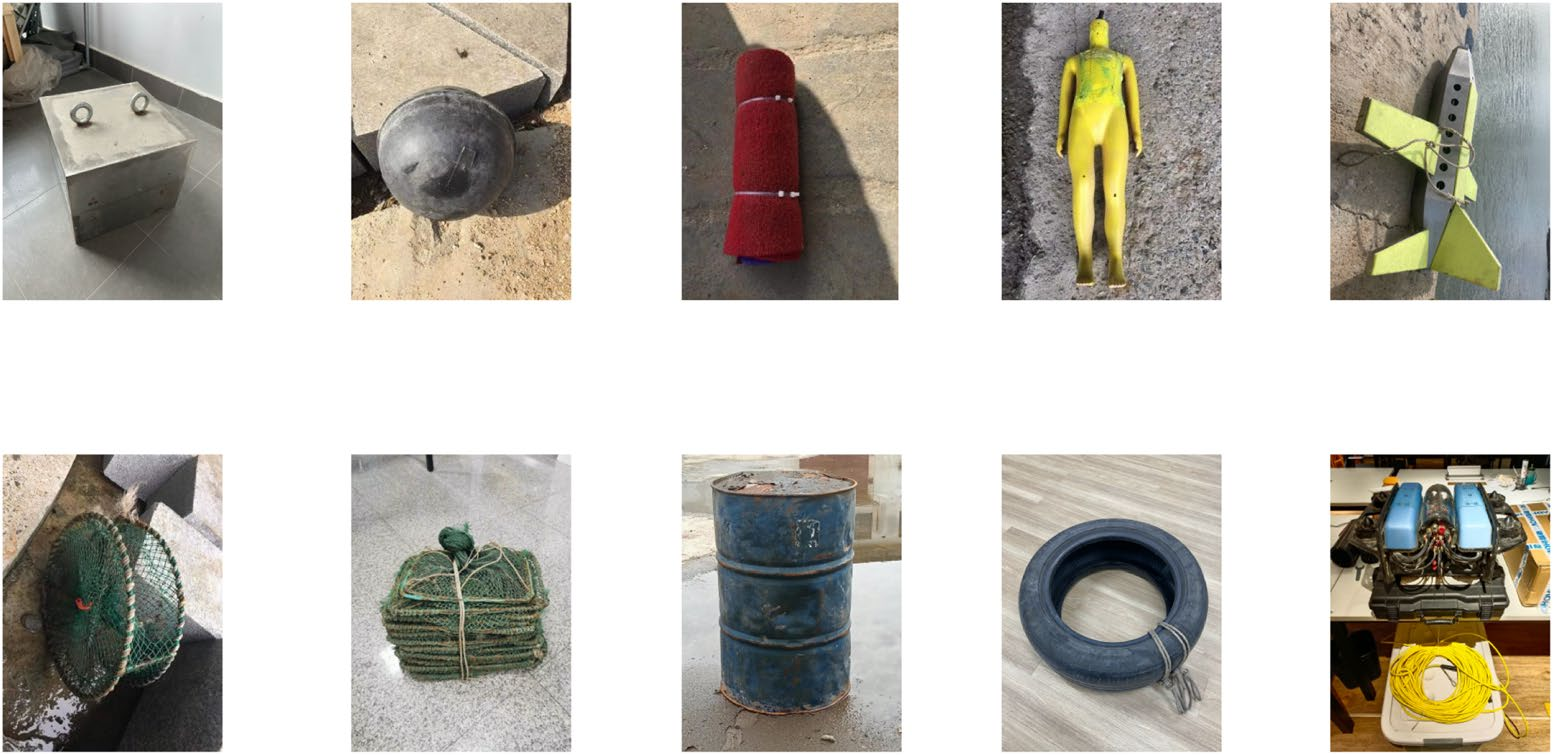
\includegraphics[width=\textwidth]{UATD_Objects.png}
    \caption[UATD Objecten.]{\label{fig:uatd_objects}Overzicht van objecten in de UATD-dataset. \autocite{Xie_2022}}
\end{figure}

De dataset wordt verspreid in een figshare-repository onder de CC BY 4.0 licentie. Deze licentie laat de gebruiker toe om het materiaal te delen en te bewerken, ook voor commerciële doeleinden. Buiten een naamsvermelding van de maker, een link naar de licentie en een vermelding of het werk al dan niet veranderd is, zijn er geen verdere restricties. De dataset wordt als ZIP-archief aangeboden. Gecomprimeerd is deze ongeveer 4,47 GB groot. Uitgepakt bevat ze drie aparte datasets en OpenSLT, de annotatietool die gebruikt werd, telkens opnieuw apart verpakt als ZIP-archief. De drie datasets zijn als volgt verdeeld: twee testsets -- \texttt{UATD\_Test\_1} en \texttt{UATD\_Test\_2} -- en één trainingsset -- \texttt{UATD\_Training}. Elk archief -- buiten die van de annotatietool natuurlijk -- bevat twee mappen: \texttt{annotations} en \texttt{images}. De map \texttt{annotations} bevat de annotaties en de map \texttt{images} bevat de sonarbeelden. \autocite{Jian_2022} \\

\begin{table}[H]
    \centering
    \begin{tabular}{llll}
        \toprule
        \textbf{Dataset} & \textbf{Aantal bestanden} & \textbf{Gecomprimeerde grootte} & \textbf{Ware grootte} \\
        \midrule
        UATD\_Test\_1  & 800  & 421.9 MB & 3.3 GB \\
        UATD\_Test\_2  & 800  & 424.6 MB & 3.3 GB \\
        UATD\_Training & 7600 & 3.9 GB   & 25.8 GB \\
        \bottomrule
    \end{tabular}
    \caption[Datasets binnen UATD]{\label{tab:uatd_datasets_overview} Tabel van eigenschappen van de datasets binnen de UATD-dataset. \autocite{Jian_2022}}
\end{table}

De bestanden volgen een vast benamingsschema zodat de beelden en de annotaties makkelijk aan elkaar gekoppeld kunnen worden. In elke dataset zijn de bestanden genummerd van \texttt{00001} tot aan het aantal bestanden in de dataset (bv. \texttt{00800} voor elke testset). Het beeld en de overeenkomstige annotatie hebben hetzelfde nummer. Zo zijn de paden voor het tweede beeld bijvoorbeeld:

\begin{itemize}
    \item \textbf{Beeld:} \texttt{UATD/UATD\_Test\_1/images/00003.bmp}
    \item \textbf{Annotatie:} \texttt{UATD/UATD\_Test\_1/annotations/00003.xml}
\end{itemize}

\begin{figure}[H]
    \centering
    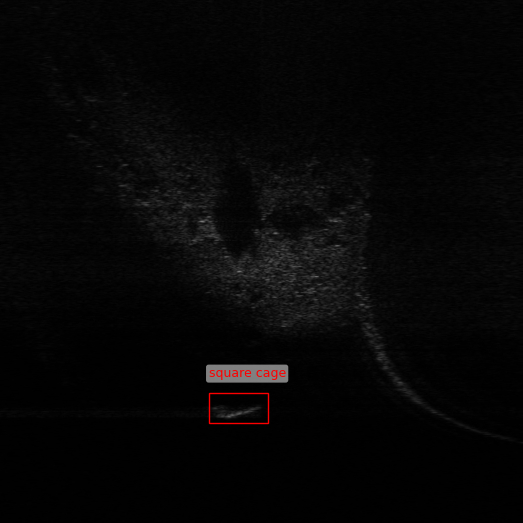
\includegraphics[width=0.5\textwidth]{UATD_example_annotated.png}
    \caption[UATD afbeelding met bounding boxes.]{\label{fig:uatd_image}Voorbeeld van een sonarbeeld binnen de UATD-dataset met de objecten aangeduid met \glspl{bounding_box} (afbeelding \texttt{UATD\_Test\_1/00003}). \autocite{Xie_2022}}
\end{figure}

De beelden zijn opgeslagen als 3-kanaals ongecomprimeerde BMP-bestanden met een bitdiepte van 8 bits (één byte). Dit is één van de eenvoudigste bestandsformaten om een foto op te slaan. Het bestand bevat namelijk een lijst van alle pixels, waarbij voor elke pixel het kleur wordt bijgehouden. Het kleur wordt in dit geval dus opgeslagen in 8 bits. Dit betekent dat het kleur van elke pixel bepaald wordt door een waarde tussen 0 en 255. Aangezien er drie kanalen zijn (RGB: Rood, Groen en Blauw), wordt elke pixel dus beschreven door $8 \times 3 = 24$ bits of 3 bytes. Als de afmetingen van de afbeelding gekend zijn, is het makkelijk om de grootte van de afbeelding te berekenen met behulp van volgende formule:

$$
\text{Grootte in Bytes} = \frac{breedte \times hoogte \times \#kanalen \times bitdiepte}{8}
$$ \\

Naast enkele tientallen bytes aan header- en fotodata is dit de werkelijke grootte van een BMP-bestand. Het nadeel is echter dat zo'n bestand heel snel heel groot wordt, aangezien BMP meestal gebruikt wordt zonder compressie. Anderzijds is zo'n verzameling van BMP-bestanden dan weer heel goed te comprimeren in bijvoorbeeld een ZIP-bestand. Zo kon de UATD-dataset van ongeveer 32,8 GB naar ongeveer 4,75 GB gecomprimeerd worden \footnote{Dit gaat over de som van de drie ZIP-bestanden die nog eens gezipt in de UATD-dataset zaten. De drie bestanden zijn dus nog eens gecomprimeerd, wat de grootte van het origineel gedownloade bestand op 4,47 GB bracht.}, wat op een compressiegraad van ongeveer 6.8 neerkomt. \autocite{Bourke_1998}

\begin{figure}[H]
    \centering
    \begin{tikzpicture}
        % Define parameters
        \def\imgSize{5}   % Image size (6x6 cm)
        \def\cellSize{1}  % Size of each cell
        \def\offset{7}    % Offset for second column
        \def\stackShift{0.5} % Shift for stacking channels
        \def\gridStep{\imgSize/5} % Step size for 6x6 grid
        
        % ==========================
        % First Column (Actual Image)
        % ==========================
        % Insert real image
        \node[anchor=south west, inner sep=0] (img) at (0,0) 
        {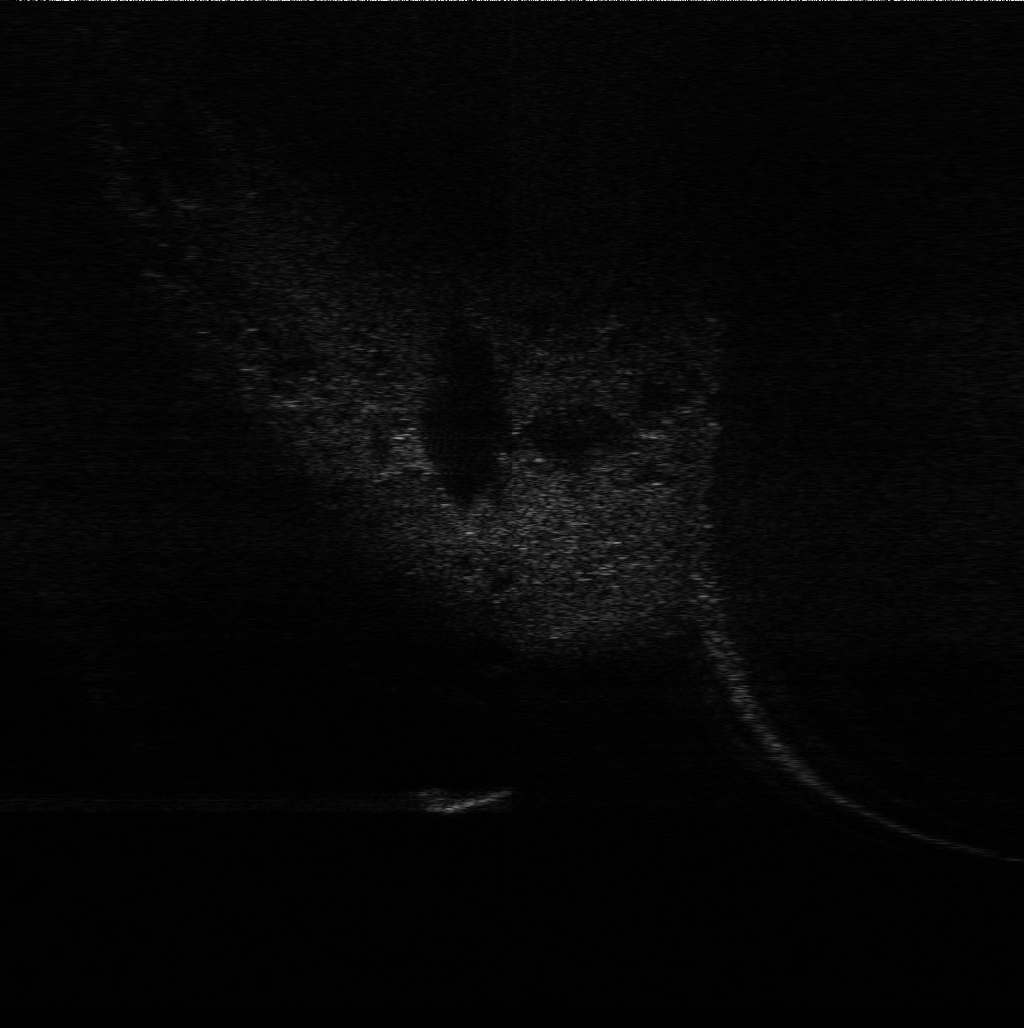
\includegraphics[width=\imgSize cm, height=\imgSize cm]{UATD_example.png}};
        
        % Draw white grid overlay (10x10)
        \draw[step=\gridStep,white, thick] (0,0) grid (\imgSize, \imgSize);
        
        % Image dimensions
        \draw[<->, thick] (-0.5, 0) -- (-0.5, \imgSize);
        \node[left] at (-0.5, \imgSize/2) {1028};
        
        \draw[<->, thick] (0, -0.5) -- (\imgSize, -0.5);
        \node[below] at (\imgSize/2, -0.5) {1024};
        
        % ==========================
        % Second Column (RGB Breakdown, Correct Stacking)
        % ==========================
        % 1. Blue Channel (furthest back, largest shift)
        \begin{scope}[shift={(\offset+2*\stackShift, 2*\stackShift)}]
            \fill[blue!50] (0,0) rectangle (\imgSize, \imgSize);
            \draw[white, thick, step=\gridStep] (0,0) grid (\imgSize, \imgSize);
        \end{scope}
        
        % 2. Green Channel (middle layer, medium shift)
        \begin{scope}[shift={(\offset+\stackShift, \stackShift)}]
            \fill[green!50] (0,0) rectangle (\imgSize, \imgSize);
            \draw[white, thick, step=\gridStep] (0,0) grid (\imgSize, \imgSize);
        \end{scope}
        
        % 3. Red Channel (front layer, no shift)
        \begin{scope}[shift={(\offset, 0)}]
            \fill[red!50] (0,0) rectangle (\imgSize, \imgSize);
            \draw[white, thick, step=\gridStep] (0,0) grid (\imgSize, \imgSize);
        \end{scope}
        
        % Dimensions for RGB squares
        \draw[<->, thick] (\offset-0.5, 0) -- (\offset-0.5, \imgSize);
        \node[left] at (\offset-0.5, \imgSize/2) {1028};
        
        \draw[<->, thick] (\offset, -0.5) -- (\offset+\imgSize, -0.5);
        \node[below] at (\offset+\imgSize/2, -0.5) {1024};
        
        % Diagonal arrow for number of channels (bottom-right corner)
        \draw[<->, thick] (\offset+0.7*\stackShift+\imgSize, -0.5) 
        -- (\offset+\stackShift+\imgSize+1, 0.5);
        \node[below] at (\offset+\stackShift+\imgSize+0.85, 0) {3};
        
    \end{tikzpicture}
    \caption[Voorbeeld van een bitmap.]{\label{fig:bitmap_example_image}Voorbeeld van de structuur van een bitmap-afbeelding zoals BMP.}
\end{figure}

Per afbeelding is er steeds een overeenkomstig XML-bestand dat de annotatie bevat. De annotatie volgt het Pascal \acrshort{voc}-formaat. Dit annotatieformaat werd origineel ontwikkeld voor de Visual Object Challenge. Deze challenge is een benchmark voor classificatie en objectdetectie die sinds 2005 jaarlijks georganiseerd wordt. Ondertussen is het formaat uitgegroeid tot een veelgebruikte standaard voor de annotatie van visuele datasets voor bijvoorbeeld objectdetectie. Door het gebruik van XML is het formaat makkelijk leesbaar. Echter maken heel weinig modellen rechtstreeks gebruik van het Pascal \acrshort{voc}-formaat, waardoor de annotatie meestal moet omgezet worden naar een ander formaat. \autocite{Everingham_2009}

\clearpage

\begin{listing}[H]
    \begin{minted}{xml}
        <annotation>
            <sonar>
                <range>24.9909</range>
                <azimuth>120</azimuth>
                <elevation>12</elevation>
                <soundspeed>1498.1</soundspeed>
                <frequency>1200k</frequency>
            </sonar>
            <file>
                <folder>UATD_Test_1</folder>
                <filename>00004</filename>
            </file>
            <size>
                <width>1024</width>
                <height>1257</height>
                <channel>3</channel>
            </size>
            <object>
                <name>rov</name>
                <bndbox>
                    <xmin>574</xmin>
                    <ymin>880</ymin>
                    <xmax>618</xmax>
                    <ymax>909</ymax>
                </bndbox>
            </object>
        </annotation>
    \end{minted}
    \caption[PASCAL VOC-annotatie]{Voorbeeld van een XML-bestand met annotatie voor objectdetectie in het PASCAL VOC-formaat (annotatie van \texttt{UATD\_Test\_1/00004}). \autocite{Xie_2022}}
\end{listing}

\subsubsection{SSS for Mine Detection}

Een andere mogelijke kandidaat is de \emph{\acrshort{sss} for Mine Detection}-dataset. Deze dataset bevat 1170 \emph{real-world} \gls{sss} sonarbeelden van de Portugese kust gemaakt door een gespecialiseerde \gls{auv}. Een dataset van deze grootte en kwaliteit verzamelen is geen sinecure, daarom is deze dataset verzameld in samenwerking met de Portugese marine. Specifiek werkten de onderzoekers gedurende verschillende jaren samen met \gls{dms3}. Dit team is verantwoordelijk voor alles wat met mijnen in zee te maken heeft. \autocite{Pessanha_Santos_2024}

\begin{figure}[H]
    \centering
    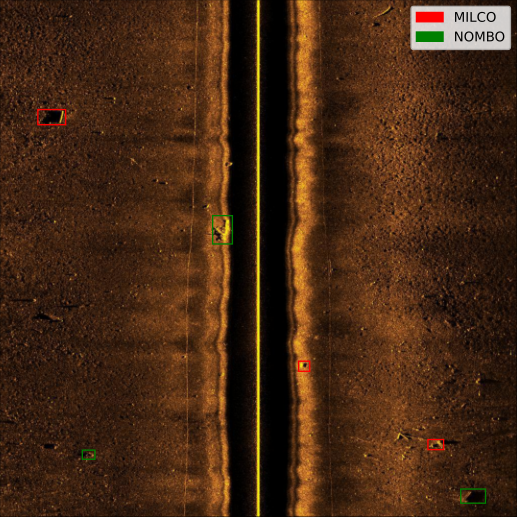
\includegraphics[width=0.5\textwidth]{SSSFMD_example_annotated.png}
    \caption[SSS for Mine Detection-afbeelding met bounding boxes.]{\label{fig:sssfmd_image}Voorbeeld van een sonarbeeld uit de \emph{\gls{sss} for Mine Detection}-dataset met de objecten aangeduid met \glspl{bounding_box} (afbeelding \texttt{SSS for Mine Detection/2015/0001\_2015}). \autocite{Pessanha_Santos_2024_SSSFMD}}
\end{figure}

Deze dataset is geschikt voor verschillende soorten ML-gerichte taken, waaronder objectdetectie, classificatie en segmentatie. De objecten in de dataset zijn geannoteerd met \glspl{bounding_box} om verschillende objecten aan te duiden. Deze vallen onder te verdelen in twee klassen: \glspl{milco} en \glspl{nombo}. Kortom: alles wat een mijn kan zijn en alles wat geen mijn kan zijn.

\begin{figure}[H]
    \centering
    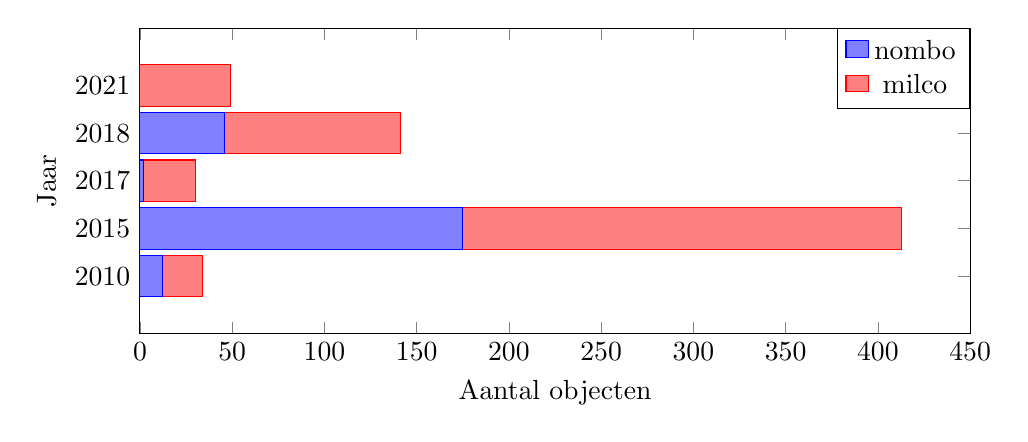
\begin{tikzpicture}
        \begin{axis}[
            xbar stacked,
            width=\textwidth,
            height=0.45\textwidth,
            symbolic y coords={2010, 2015, 2017, 2018, 2021},
            ytick=data,
            xmin=0,
            xmax=450,
            bar width=15pt,
            enlarge y limits=0.3,
            legend style={at={(1,1)}, anchor=north east, legend columns=1},
            xlabel={Aantal objecten},
            ylabel={Jaar}
            ]
            % First column data (Bottom part of stacked bars)
            \addplot+[xbar, color=blue, fill=blue!50] coordinates {(12,2010) (175,2015) (2,2017) (46,2018) (0,2021)};
            \addlegendentry{\glspl{nombo}}
            
            % Second column data (Top part of stacked bars)
            \addplot+[xbar, color=red, fill=red!50] coordinates {(22,2010) (238,2015) (28,2017) (95,2018) (49,2021)};
            \addlegendentry{\glspl{milco}}
            
        \end{axis}
    \end{tikzpicture}
    \caption[Aantal objecten per jaar in SSS for Mine Detection.]{\label{fig:SSSFMD_objects_per_year}Grafiek van het aantal waargenomen objecten per jaar in de \emph{\gls{sss} for Mine Data}-dataset. \autocite{Pessanha_Santos_2024}}
\end{figure}

Ook deze dataset wordt verspreid in een figshare-repository onder de CC BY 4.0 licentie. Opnieuw wordt een ZIP-archief van ongeveer 584 MB aangeboden. Dit ZIP-archief bevat opnieuw andere ZIP's. Deze hebben de naam van één van de jaren waarvan er data beschikbaar is en bevatten dit dan ook. Daarnaast is er nog een ZIP-bestand met de gewichten van een getraind \gls{YOLO}v4-model en de code hiervoor. Dit is echter niet nuttig voor dit onderzoek en zal dus niet gebruikt worden. \\

In de mappen verdeeld per jaar zitten zowel de beelden als de annotaties (niet gescheiden). De beelden zijn JPG-bestanden. Het lijkt erop dat er twee verschillende resoluties gebruikt zijn voor de afbeeldingen, namelijk \texttt{416 x 416} en \texttt{1024 x 1024}. De afbeeldingen volgen een vast benamingsschema: elke afbeelding bevat een oplopend nummer beginnend van \texttt{0001}, daarna een underscore en dan het jaar waarin de afbeelding is gemaakt. Alles samen is dat dus bijvoorbeeld: \texttt{0001\_2015.jpg}. De bestanden met annotatie staan in dezelfde map en hebben dezelfde naam als hun overeenkomstige afbeeldingen. Het enige verschil is dat zij een \texttt{.txt}-extensie hebben. Dit tekstbestand bevat de annotatie in \gls{yolo}-formaat. \autocite{Pessanha_Santos_2024_SSSFMD}

\begin{listing}[H]
    \begin{minted}{text}
        0 0.10009765625 0.2265625 0.0537109375 0.029296875
        1 0.43017578125 0.4443359375 0.0380859375 0.0546875
        0 0.587890625 0.7080078125 0.021484375 0.01953125
        0 0.84228515625 0.859375 0.0302734375 0.01953125
        1 0.17138671875 0.87890625 0.0244140625 0.017578125
        1 0.91455078125 0.958984375 0.0478515625 0.02734375
    \end{minted}
    \caption[YOLO-annotatie]{Voorbeeld van een TXT-bestand met annotatie voor objectdetectie in het YOLO-formaat (annotatie van \texttt{SSS for Mine Detection/2015/0001\_2015}). \autocite{Pessanha_Santos_2024_SSSFMD}}
\end{listing}

Eigenlijk is dit niks meer dan een CSV-bestand waarbij de separator een spatie is. In getabelleerde vorm is de data iets overzichtelijker.

\begin{table}[H]
    \centering
    \begin{tabular}{lllll}
        \toprule
        \textbf{Klasse} & \textbf{$x$-coördinaat} & \textbf{$y$-coördinaat} & \textbf{Hoogte} & \textbf{Breedte} \\
        \midrule
        0 & 0.10009765625 & 0.2265625    & 0.0537109375 & 0.029296875 \\
        1 & 0.43017578125 & 0.4443359375 & 0.0380859375 & 0.0546875   \\
        0 & 0.587890625   & 0.7080078125 & 0.021484375  & 0.01953125  \\
        0 & 0.84228515625 & 0.859375     & 0.0302734375 & 0.01953125  \\
        1 & 0.17138671875 & 0.87890625   & 0.0244140625 & 0.017578125 \\
        1 & 0.91455078125 & 0.958984375  & 0.0478515625 & 0.02734375  \\
        \bottomrule
    \end{tabular}
    \caption[YOLO-annotatie in getabelleerde vorm]{\label{tab:yolo_annot_table} Tabel met annotatie voor objectdetectie in het YOLO-formaat (annotatie van \texttt{SSS for Mine Detection/2015/0001\_2015}). \autocite{Pessanha_Santos_2024_SSSFMD}}
\end{table}

Merk op dat de klasse \texttt{0} of \texttt{1} is. Uit de paper van \textcite{Pessanha_Santos_2024} blijkt dat \texttt{0} een \gls{milco} is en \texttt{1} een \gls{nombo}. De volgende vier kolommen stellen een \gls{bounding_box} voor. Er bestaan verschillende formaten om zo'n \gls{bounding_box} voor te stellen. Dit formaat gebruikt één coördinaat ($(x, y)$) die het midden van de \gls{bounding_box} voorstelt, de hoogte en de breedte. \\

Men zou verwachten dat deze waarden gegeven zijn in pixels. Dat brengt echter een probleem met zich mee wanneer de afbeelding geschaald wordt. Dan moeten de pixelwaarden telkens herberekent worden om zo de \gls{bounding_box} op de juiste plaats op de afbeelding te laten vallen. Om dit op te lossen worden deze waarden -- zoals hier -- meestal als verhoudingen uitgedrukt. Zo is de breedte bijvoorbeeld de breedte in pixels gedeeld door de breedte van de afbeelding.

\begin{figure}[H]
    \centering
    \begin{tikzpicture}
        
        % Draw the outer rectangle (image)
        \draw[thick] (0,0) rectangle (7,7);
        % Label the dimensions of the outer rectangle
        \draw[<->] (-0.5,0) -- (-0.5,7) node[midway, left] {$h_{image}$};
        \draw[<->] (0,-0.5) -- (7,-0.5) node[midway, below] {$w_{image}$};
        
        % Draw the bounding box inside the image
        \draw[thick, dashed] (2,2) rectangle (5,5);
        % Label the dimensions of the bounding box
        \draw[<->] (1.5,2) -- (1.5,5) node[midway, left] {$h_{bb}$};
        \draw[<->] (2,1.5) -- (5,1.5) node[midway, below] {$w_{bb}$};
        
        % Add a dot in the center of the bounding box
        \filldraw [black] (3.5,3.5) circle (2pt);
        % Label the coordinates of the dot
        \node at (3.5,3) {$(x_{bb}, y_{bb})$};
        
    \end{tikzpicture}
    \caption[Structuur van een bounding box.]{\label{fig:bounding_box}Structuur van een \gls{bounding_box} (gebaseerd op een figuur van \textcite{Pessanha_Santos_2024})}.
\end{figure}

Als de afbeelding geschaald wordt, schaalt de \gls{bounding_box} mee en kan men aan de hand van een relatief eenvoudige formule terug de pixelwaarde berekenen zonder complexe transformaties op de \gls{bounding_box} te moeten gaan toepassen. De formule om de absolute pixelwaarden om te zetten naar relatieve verhoudingen is de volgende:

$$
(x,y,w,h) = \left(\frac{x_{bb}}{w_{image}},\frac{y_{bb}}{h_{image}},\frac{w_{bb}}{w_{image}},\frac{h_{bb}}{h_{image}}\right)
$$ 

\clearpage

Naast het verzamelen van de dataset trainden de onderzoekers ook een objectdetectiemodel -- namelijk \gls{yolo}v4 -- op deze data om de kwaliteit ervan te testen. De configuratie voor het trainingsproces werd speciaal aangepast om de performance van dit model te verhogen. De \gls{batch_size} werd ingesteld op 64 en werden gedurende de training opgesplitst in 16 \glspl{mini_batch} van elk 4 afbeeldingen, dit om het geheugengebruik tijdens het trainingsproces te optimaliseren. \\

Het maximum aantal \glspl{batch} werd ingesteld op 6000. Ook werd de \gls{learning_rate} van het model op kritieke punten aangepast, namelijk na het verwerken van 4800 en 5400 \glspl{batch}, dit om de convergentie te verhogen. Ook pasten de onderzoekers transfer learning toe door de gewichten van het model te initialiseren met gewichten van de \gls{coco}-dataset. Na het model te trainen op de volledige dataset van 1170 afbeeldingen, behaalde deze een \gls{iou} van 60\% en een \gls{map} van 75\%. Ook werd een \gls{precision} van 82\% en een \gls{recall} van 64\% behaald. \autocite{Pessanha_Santos_2024}

\subsubsection{UXO}

Ten slotte is er de \acrshort{uxo}-dataset. \acrshort{uxo} is de afkorting voor \acrlong{uxo}, de Engelse benaming voor \glspl{blindganger}. Dit is meteen ook de inhoud van deze dataset. Ze bevat namelijk 74 437 afbeeldingen van \glspl{blindganger} en is daarmee de grootste dataset die in dit onderzoek voorkomt. Het doel van deze dataset is om een validatieset te zijn en ze is samengesteld om onderzoek naar ontmijning in plassen, meren, zeeën en oceanen vooruit te helpen. Zoals al eerder vermeld is dit onderwerp zeer gevoelig en wordt er meestal (lees: bijna altijd) voor gekozen om deze datasets zo confidentieel mogelijk te houden. Daarom bevat deze dataset ook geen \emph{real-world}-afbeeldingen. In plaats daarvan zijn beelden in een gecontroleerde, experimentele omgeving gemaakt. \autocite{Dahn_2024_UXO}

\begin{figure}[H]
    \centering
    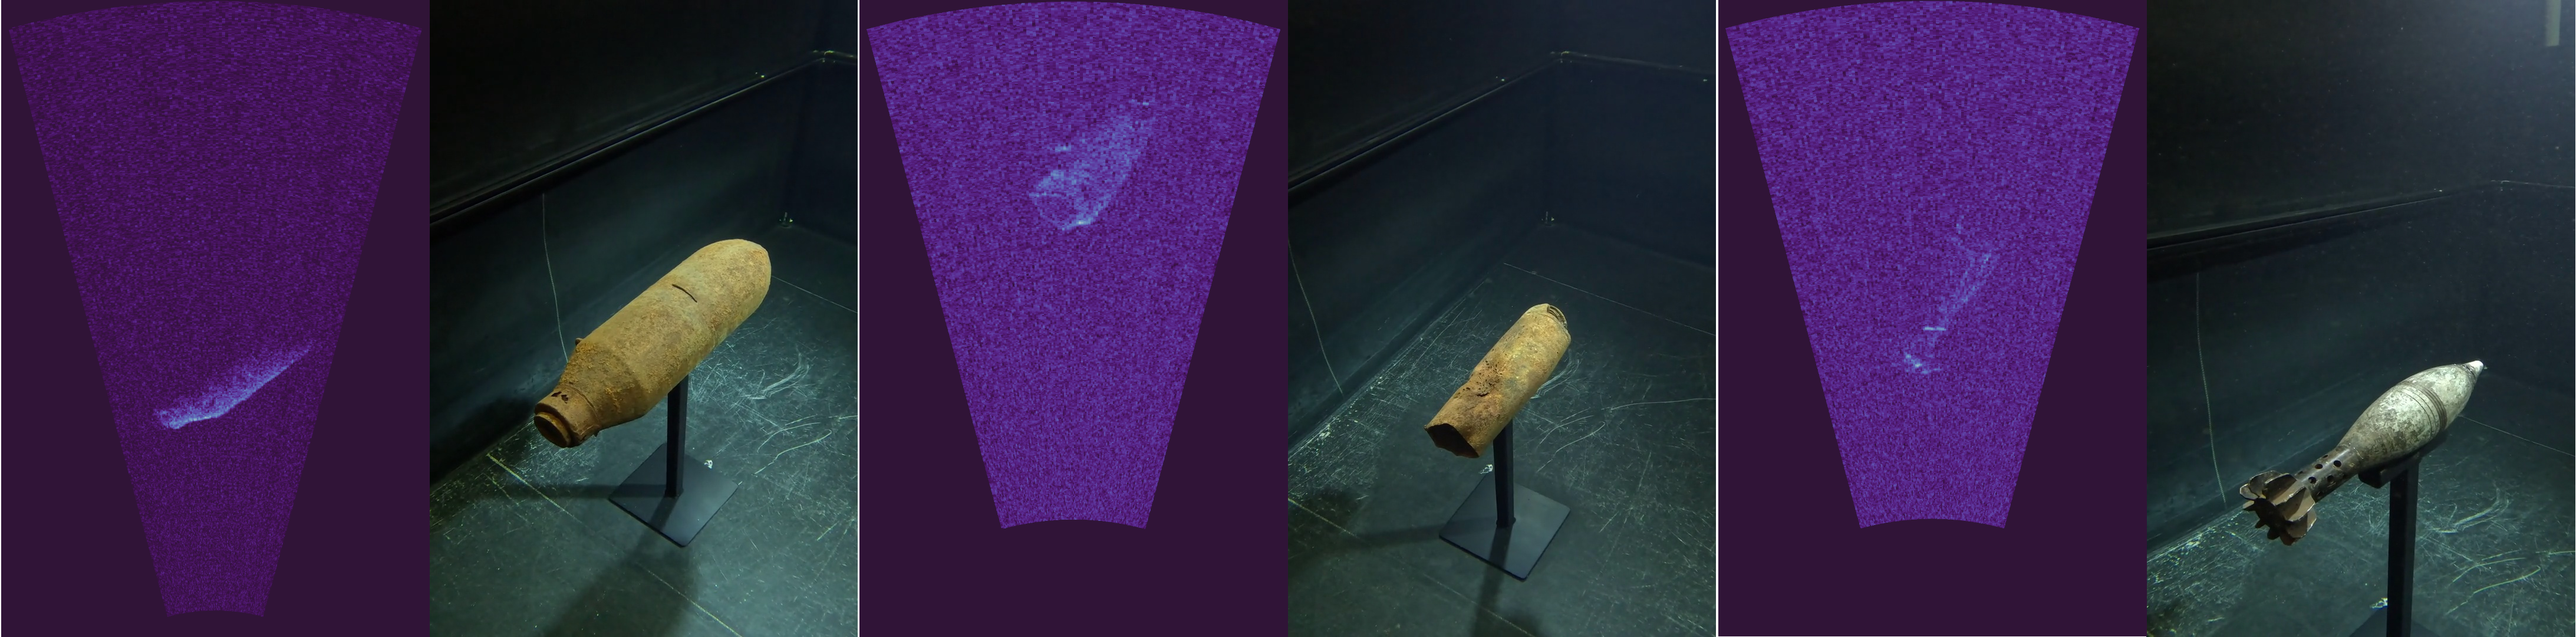
\includegraphics[width=\textwidth]{teaser_uxo.png}
    \caption[Voorbeeld van sonarbeelden \& afbeeldingen in de UXO-dataset]{\label{fig:uxo_teaser}. Voorbeeld van sonarbeelden en overeenkomstige afbeeldingen van verschillende type \glspl{blindganger} in de UXO-dataset. \autocite{Dahn_2024_UXO}}
\end{figure}

Om deze dataset samen te stellen, hebben de onderzoekers een volledig gecontroleerde testopstelling gemaakt bij het \gls{dfki}, het Duits onderzoekscentrum voor artificiële intelligentie in Bremen. De dataset is gemaakt met een ARIS Explorer 3000 sonarmodule (voor de sonarbeelden) en een GoPro Hero 8 (voor de bijhorende 5,3K UHD afbeeldingen). Deze twee modules werden op een \gls{PTU} (de ARIS Rotator AR3) gemonteerd die vastzat aan een op maat gemaakte \gls{portaalkraan}. Deze kraan kon vrij in de $xyz$-assen bewegen en kon verschillende voorgeprogrammeerde banen heel precies volgen. 

\begin{figure}[H]
    \centering
    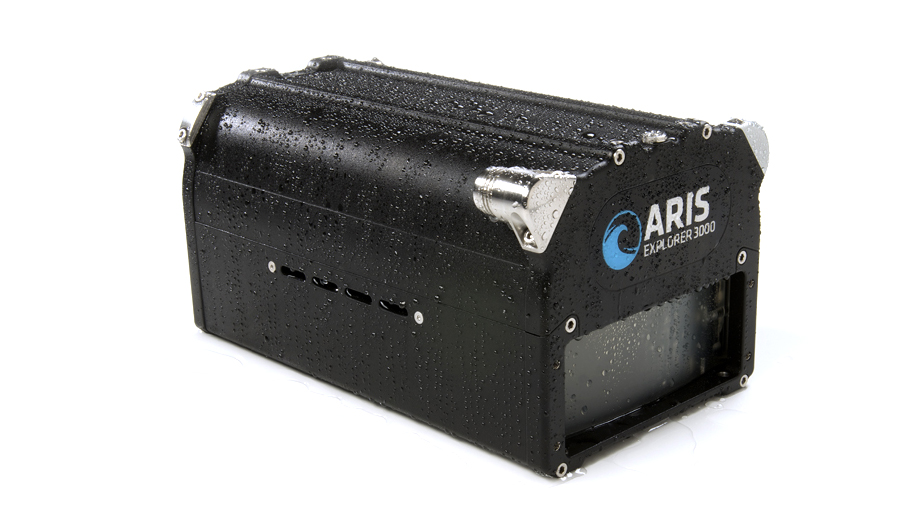
\includegraphics[width=0.5\textwidth]{ARIS-3000.jpg}
    \caption[Afbeelding van de ARIS Explorer 3000]{\label{fig:aris_3000}. Afbeelding van de ARIS Explorer 3000 sonarmodule. \autocite{soundmetrics.com}}
\end{figure}

Om de omgeving van de zee zo goed mogelijk te kunnen nabootsen, bouwden de onderzoekers een bassin gevuld met 20 000 liter zoetwater. Hierin plaatsten ze verschillende \emph{targets}, de \glspl{blindganger}. Deze waren aangeleverd door EGGERS Kampfmittelbergung GmbH, een bedrijf dat zich bezighoudt met het ontmijnen van verschillende sites. Om de veiligheid te garanderen, werden de \glspl{blindganger} voordien onschadelijk gemaakt. Er werden verschillende \glspl{blindganger} gebruikt om zo variëteit in de dataset te garanderen: een normale bom van ongeveer 51 kg, een vervormde fosforbom en een mortier. \autocite{Dahn_2024}

\begin{figure}[H]
    \centering
    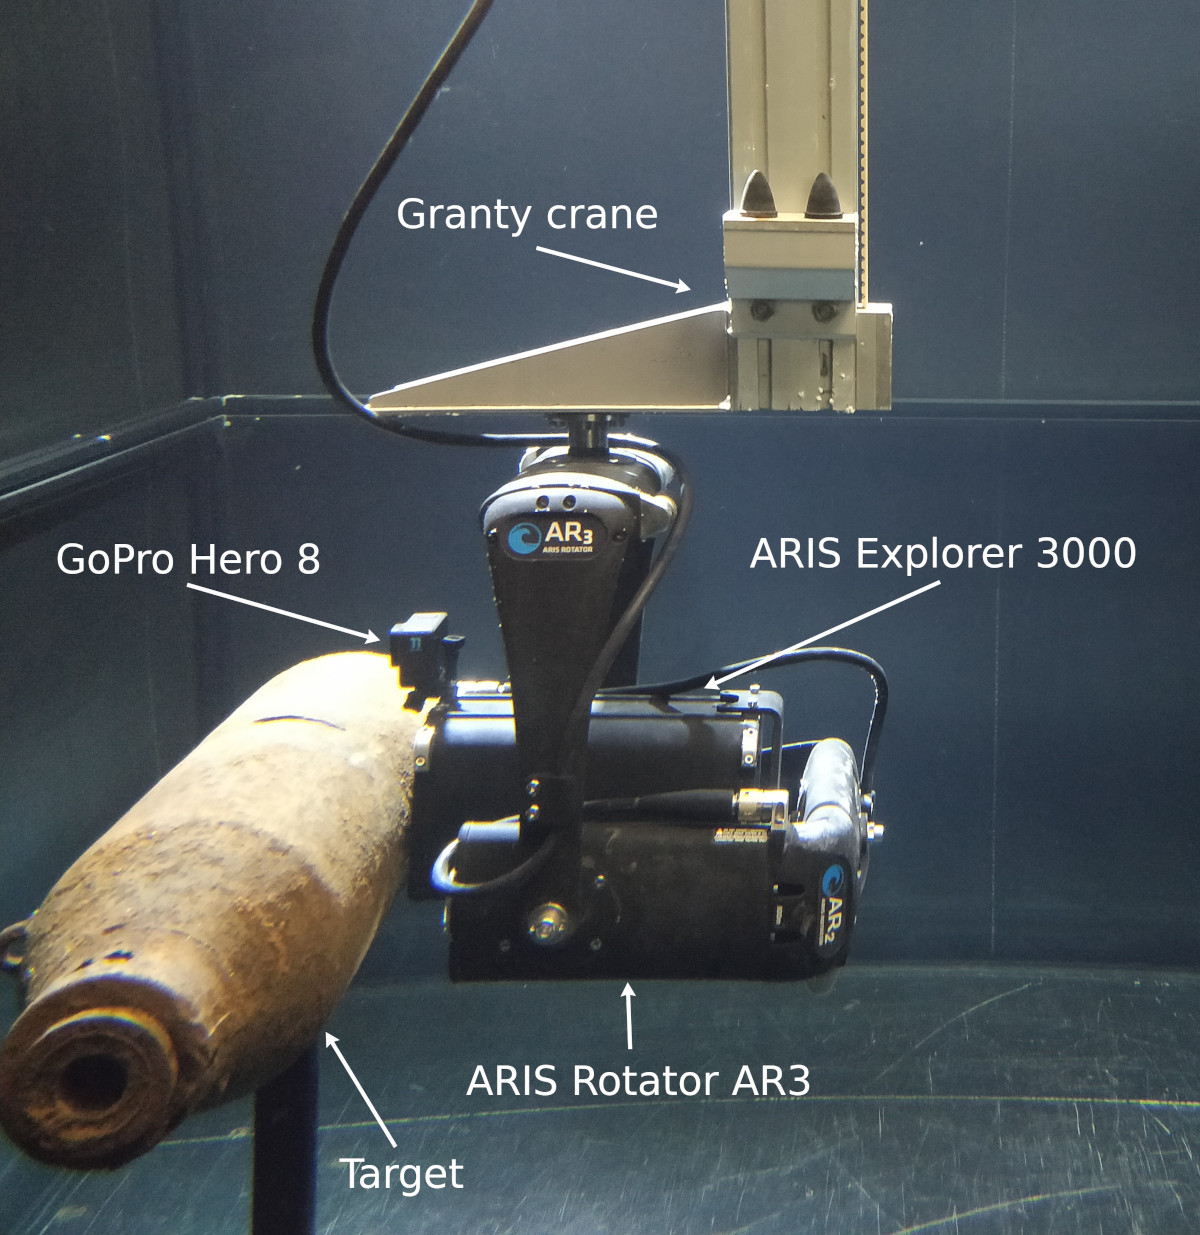
\includegraphics[width=0.5\textwidth]{uxo_setup.jpg}
    \caption[Setup waarmee de UXO-dataset gemaakt is]{\label{fig:uxo_setup}. Afbeelding van de setup die gebruikt werd om data te verzamelen voor de UXO-dataset. \autocite{Dahn_2024_UXO}}
\end{figure}

De dataset is alles samen zo'n 94,7 GB groot. Ze is de meest uitgebreide die in dit onderzoek voorkomt, niet alleen qua grootte, maar ook qua inhoud. De dataset is onderverdeeld in verschillende mappen. De map \texttt{3d\_models} bevat 3D-modellen van de \glspl{blindganger}. De map \texttt{calibration} bevat dan weer de transformaties tussen de kraan en de sensors en de kalibraties van de GoPro. Het merendeel van de dataset zit in de map \texttt{recordings}. Deze bevat mappen per type \gls{blindganger}. In deze mappen zitten dan telkens weer mappen met de datum en tijd van elk experiment. Deze mappen bevatten verschillende mappen en bestanden die de \emph{core} van de data vormen. \autocite{Dahn_2024_UXO}

\clearpage

\begin{itemize}
    \item \textbf{\texttt{aris\_raw}:} map die de \emph{raw} sonarbeelden bevat in PGM formaat. Dit is een eenvoudig rasterafbeeldingsformaat (zoals BMP, cf. figuur \ref{fig:bitmap_example_image}) dat grijswaardenafbeeldingen opslaat. PGM-bestanden kunnen in een ASCII (tekst) of binaire (snellere) variant worden opgeslagen. Elke pixel heeft een intensiteitswaarde tussen 0 (zwart) en een maximumwaarde (meestal 255, wit), waardoor verschillende grijstinten mogelijk zijn. De afbeelding bevat ook een header met het formaat, afmetingen en maximale intensiteit, gevolgd door de pixelgegevens. PGM wordt vaak gebruikt in beeldverwerking en wetenschappelijke toepassingen vanwege de eenvoud en brede compatibiliteit. \autocite{Poskanzer_2016}
    \item \textbf{\texttt{aris\_polar}:} map die de poolgetransformeerde sonarbeelden bevat in PNG formaat.
    \item \textbf{\texttt{gopro}:} map die de beelden in JPG formaat bevat die gemaakt zijn door de GoPro.
    \item \textbf{\texttt{labels}:} map die annotatie van \glspl{bounding_box} bevat in JSON formaat.
    \item \textbf{\texttt{aris\_file\_meta.yaml}:} YAML-bestand met de metadata van de sonar 
    \item \textbf{\texttt{aris\_frame\_meta.csv}:} CSV-bestand met metadata voor elk sonarframe, inclusief \gls{ptu}-informatie.
    \item \textbf{\texttt{gantry.csv}:} CSV-bestand met posities van de \gls{portaalkraan} bij elk sonarframe.
    \item \textbf{\texttt{notes.txt}:} TXT-bestand met korte beschrijving over experiment.
\end{itemize}

\begin{figure}[H]
    \centering
    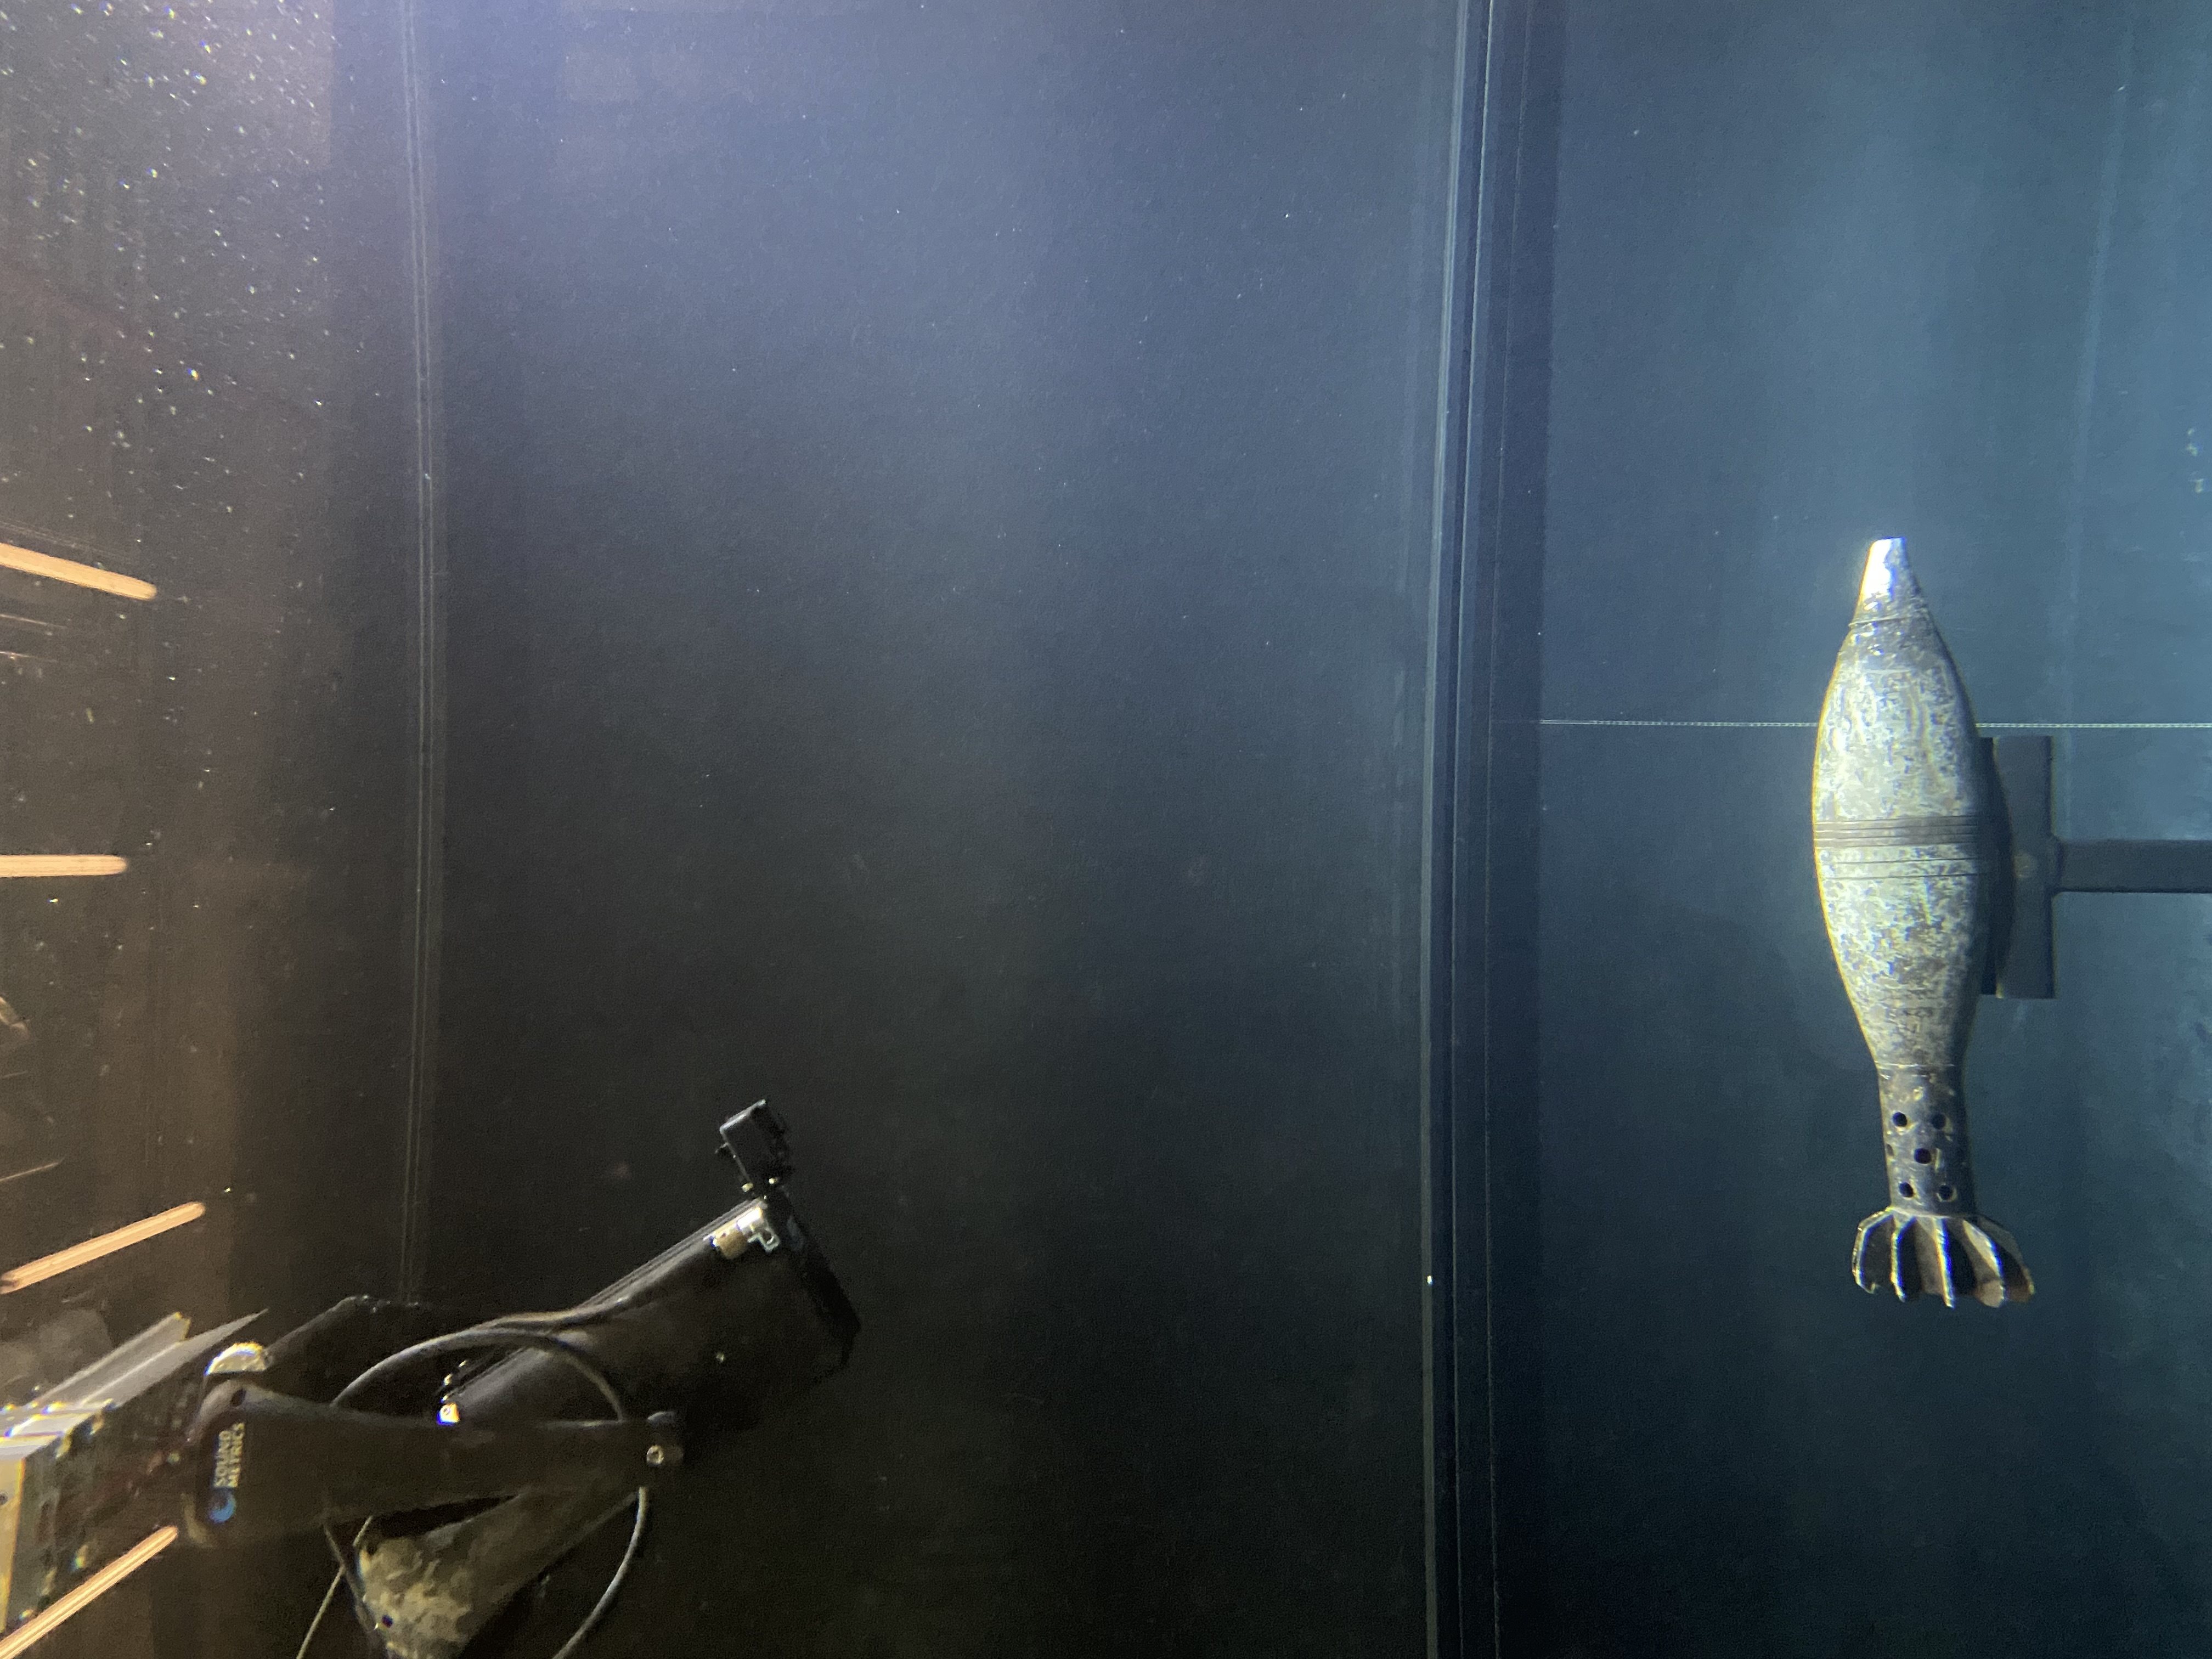
\includegraphics[width=0.5\textwidth]{uxo_preview.jpg}
    \caption[UXO-setup in actie]{\label{fig:uxo_preview}. Preview van de setup waarmee de UXO-dataset is gemaakt in actie. \autocite{Dahn_2024_UXO}}
\end{figure}

\clearpage

\subsubsection{Conclusie}

Alle drie de datasets die hierboven besproken werden, maken het mogelijk om een objectdetectiemodel mee te trainen. Ze bieden namelijk allemaal annotaties van \glspl{bounding_box} op de bijhorende afbeeldingen aan. Daarnaast zijn deze datasets makkelijk te verwerken, aangezien alle beelden in conventionele afbeeldingsformaten zijn opgeslagen (zoals PNG, JPG, BMP, PGM, \dots). Toch is er -- specifiek voor dit onderzoek -- één dataset die geschikter is dan de anderen. De UATD-dataset is -- misschien ietwat subjectief -- uitgekozen om te gebruiken in de rest van dit onderzoek. Dit komt omdat ze bepaalde aspecten aanbiedt die de andere datasets niet hebben. \\

\gls{sss} for Mine Detection lijkt op het eerste zicht de perfecte dataset voor dit onderzoek. Het probleem is echter dat ze relatief klein is: ze bevat ``slechts'' 1170 afbeeldingen. Op het eerste zicht lijkt dit voldoende. Echter moet deze dataset nog opgesplitst worden in -- ten minste -- een trainingsset en een testset.\footnote{In een optimale situatie zou de data opgesplitst worden in drie sets: een trainingsset, een testset en een validatieset. Dit komt omdat de validatiedataset -- hoewel ze niet gebruikt wordt om het model te trainen -- gebruikt wordt om de paramaters van het model te tunen. Dit kan leiden tot \gls{overfitting}. Het is beter om als testset data te gebruiken dat het model nog niet gezien heeft. \autocite{Goodfellow_2016}} Ook komen er slechts 668 objecten voor in de dataset. Tot overmaat van ramp zijn deze ook zeer slecht verdeeld. 

\begin{table}[H]
    \centering
    \begin{tabular}{ll}
        \toprule
        \textbf{\# objecten / beeld} & \textbf{\# beelden} \\
        \midrule
        13 & 1 \\
        9  & 2 \\
        8  & 4 \\
        7  & 8 \\
        6  & 8 \\
        5  & 13 \\
        4  & 9 \\
        3  & 41 \\
        2  & 59 \\
        1  & 159 \\
        0  & 866 \\
        \bottomrule
    \end{tabular}
    \caption[Aantal objecten per afbeelding in SSS for Mine Data]{\label{tab:objects_per_image_sss} Tabel met verdeling van objecten per afbeelding in de \gls{sss} for Mine Detection-dataset.}
\end{table}

\clearpage

Er is één afbeelding met wel 13 objecten en 866 zonder ook maar één object. Door deze slechte verdeling en de beperkte hoeveelheid data in de dataset is ze dus weinig bruikbaar voor dit onderzoek. \\

Dit is een probleem waar de UXO-dataset absoluut niet mee kampt. Deze heeft dan echter weer andere problemen. De dataset is namelijk volledig samengesteld in een gecontroleerde testopstelling. Ze bevat dus geen \emph{real-world}-data. Dit betekent echter ook dat bepaalde artefacten en afwijkingen typisch aan meren en zeeën niet in deze dataset voorkomen. De beelden zijn zodanig zuiver dat het hoogstwaarschijnlijk mogelijk zou zijn om de \glspl{blindganger} te herkennen door te zoeken naar de groep helderste pixels of met een edge-detection algoritme. \autocite{Torre_1986} \\

Ook de grootte van de dataset is misschien iets te mooi om waar te zijn. De beelden in de dataset zijn namelijk geen onafhankelijke afbeeldingen, maar frames van een continue opname. Dit zorgt ervoor dat er (nagenoeg) geen verschil is tussen afbeelding $n$ en afbeelding $n+1$. Als alle afbeeldingen na elkaar worden afgespeeld, ziet men een opname van een transformatie (rotatie, verschuiving, \dots) van één van de \glspl{blindganger}. Ten slotte staat er telkens maar één object op een afbeelding, wat multiple objectdetectie (meerdere objecten op één afbeelding herkennen) onmogelijk maakt.